% Single-column adaptation of CVPR typography; not an official submission layout.
\documentclass[10pt,letterpaper]{article}
\usepackage[letterpaper,textwidth=7.1in,textheight=9.25in,top=.8in,left=.7in]{geometry}
\usepackage[T1]{fontenc}
\usepackage{mathptmx,helvet,courier,microtype,amsmath,amssymb,booktabs,graphicx,array,tabularx}
\usepackage[font=small,labelfont=bf,labelsep=period,skip=5pt,justification=justified,singlelinecheck=false]{caption}
\usepackage{enumitem,placeins,xcolor}
\usepackage[numbers,sort&compress]{natbib}
\usepackage[colorlinks=true,linkcolor=black,citecolor=black,urlcolor=blue!45!black]{hyperref}
\usepackage{titlesec}
\titleformat{\section}{\fontsize{12}{14}\selectfont\bfseries}{\thesection.}{.5em}{}
\titleformat{\subsection}{\fontsize{10}{12}\selectfont\bfseries}{\thesubsection.}{.5em}{}
\titlespacing*{\section}{0pt}{11pt plus 2pt minus 1pt}{5pt}
\titlespacing*{\subsection}{0pt}{8pt plus 1pt}{4pt}
\setlength{\parindent}{0pt}
\setlength{\parskip}{4pt plus 1pt minus 1pt}
\setlength{\textfloatsep}{11pt plus 2pt minus 2pt}
\setlength{\floatsep}{9pt plus 2pt minus 2pt}
\setlength{\intextsep}{10pt plus 2pt minus 2pt}
\setlength{\abovecaptionskip}{5pt}
\setlength{\belowcaptionskip}{0pt}
\renewcommand{\arraystretch}{1.08}
\renewcommand{\topfraction}{.9}
\renewcommand{\bottomfraction}{.8}
\renewcommand{\textfraction}{.08}
\renewcommand{\floatpagefraction}{.75}
\setcounter{topnumber}{3}
\setcounter{bottomnumber}{2}
\setcounter{totalnumber}{5}
\setlist{nosep,leftmargin=*}
\pagestyle{plain}
\frenchspacing
\clubpenalty=10000
\widowpenalty=10000
\displaywidowpenalty=10000
\raggedbottom
\title{Beyond Skip Counts:\\Understanding Adaptive Caching for Efficient Generation}
% Names, order and email addresses transcribed from the group list supplied by the user.
\author{\begin{tabular*}{\textwidth}{@{\extracolsep{\fill}}cccc@{}}
HAN SHUANGYUE\textsuperscript{*} & JIANG NAN\textsuperscript{*} & WANG HAIZHOU\textsuperscript{*} & YAN XINYU\textsuperscript{*}\\[3pt]
{\fontsize{8}{10}\selectfont\texttt{hans0053@e.ntu.edu.sg}} &
{\fontsize{8}{10}\selectfont\texttt{njiang005@e.ntu.edu.sg}} &
{\fontsize{8}{10}\selectfont\texttt{c250281@e.ntu.edu.sg}} &
{\fontsize{8}{10}\selectfont\texttt{xinyu039@e.ntu.edu.sg}}
\end{tabular*}\\[5pt]{\fontsize{8}{10}\selectfont\textsuperscript{*}Equal contribution.}}

\date{}
\makeatletter
\setlength{\@fptop}{0pt}
\setlength{\@fpsep}{12pt}
\setlength{\@fpbot}{0pt plus 1fil}
\renewcommand{\maketitle}{\begin{center}
{\fontsize{15}{18}\selectfont\bfseries\@title\par}\vspace{9pt}
{\fontsize{11}{13}\selectfont\@author\par}\vspace{10pt}
\end{center}}
\renewenvironment{abstract}{\begin{center}\bfseries\fontsize{12}{14}\selectfont Abstract\end{center}\vspace{-4pt}\begin{quote}\small\setlength{\parindent}{0pt}\noindent}{\end{quote}\vspace{5pt}}
\makeatother
\hypersetup{pdftitle={Beyond Skip Counts: Understanding Adaptive Caching for Efficient Generation},pdfsubject={CE6190 Group Project: When to Reuse in Image and Video Generation},pdfauthor={Han Shuangyue; Jiang Nan; Wang Haizhou; Yan Xinyu}}
\begin{document}
\maketitle
\begin{abstract}
Iterative image and video generation is computationally expensive because each sampling step evaluates a large neural network.
Caching enables efficient generation without retraining by reusing intermediate computations whose changes are small enough to tolerate.
We study when to reuse cached features and when to recompute them.
We establish a controlled benchmark of Uncached, TeaCache, MagCache, SeaCache, and SenCache across text-to-image and text-to-video generation, evaluating reference fidelity, content quality, and measured generation time.
Policies with the same computation count and nearly identical runtime can still differ substantially in fidelity to Uncached.
Compared with TeaCache, MagCache reduces LPIPS distance to Uncached by 40.3\% on Wan2.1, while SenCache reduces it by 51.2\% on FLUX.1-dev.
On FLUX.1-dev, SeaCache has lower LPIPS than SenCache near $1.7\times$ speedup, while SenCache has lower LPIPS near $2.45\times$.
We examine these decisions through component ablations, recorded computation schedules, and mathematical analysis.
In one SenCache setting, all 200 FLUX prompts recompute at the same 11 of 28 sampling steps.
After the early stages, every recomputation is forced by the consecutive-reuse limit, so increasing the main threshold cannot reduce computation further.
\end{abstract}

\section{Introduction}
Iterative image and video generation is computationally expensive because a large neural network is evaluated repeatedly along the sampling trajectory.
Caching reduces this cost by reusing intermediate features that change slowly between nearby sampling stages~\cite{ma2024deepcache,liu2025teacache,kahatapitiya2025adacache}.
For diffusion transformers~\cite{peebles2023dit}, reusing these features avoids expensive block computations while retaining the sampler's latent updates.
We focus on deciding when to reuse these features and when a fresh computation is necessary.

SeaCache~\cite{chung2026seacache} and SenCache~\cite{haghighi2026sencache} address this decision using spectral and sensitivity-based signals, respectively; TeaCache~\cite{liu2025teacache} and MagCache~\cite{ma2025magcache} provide established alternatives.
Comparing these policies requires more than counting skipped computations.
Their thresholds have different scales, equal computation counts can allocate work to different stages, and protection rules can override an otherwise adaptive gate.
We therefore ask how much fidelity each policy preserves at a measured generation budget, and which decisions determine that outcome.

We establish a controlled benchmark in two parallel settings: FLUX.1-dev~\cite{flux2024} on DrawBench~\cite{saharia2022imagen} and Wan2.1~\cite{wan2025wan} on a VBench~\cite{huang2024vbench} subset.
Within each backbone, the methods share residual reuse and cache scope, with outputs paired against Uncached references.
We compare measured time and reference fidelity, assess content quality separately, and examine component ablations and decision traces to explain the observed trade-offs.
Our contributions are threefold:
\begin{enumerate}[label=(\arabic*),topsep=3pt,itemsep=3pt]
\item \textbf{A controlled benchmark for adaptive caching.}
We compare five methods across image and video generation using paired references, runtime measurements, threshold sweeps, and complementary quality metrics, with recorded configurations and traceable evidence.\footnote{Project repository: \url{https://github.com/AvianHan/CE6190-Visual-Generation}.}
\item \textbf{Empirical findings beyond skip counts.}
At matched computation counts and nearly identical runtime, MagCache reduces Wan LPIPS by 40.3\% relative to TeaCache, while SenCache reduces FLUX LPIPS by 51.2\%.
SeaCache and SenCache also achieve lower LPIPS at different measured FLUX speedups.
\item \textbf{Mechanistic and mathematical analysis.}
Component ablations and computation schedules reveal how decision signals and reuse limits affect the allocation of computation.
We prove that equal computation counts can produce different errors, and derive the minimum computation count imposed by a consecutive-reuse limit.
\end{enumerate}

\clearpage
\section{Related Work}
\label{sec:related}
\subsection{Efficient Generation}
Diffusion models~\cite{ho2020ddpm} and score-based models~\cite{song2021sde} construct samples through iterative denoising; Flow Matching~\cite{lipman2023flowmatching} and rectified flow~\cite{liu2023rectifiedflow} learn vector fields connecting noise and data.
Latent diffusion~\cite{rombach2022ldm} lowers the cost of the representation, while diffusion transformers~\cite{peebles2023dit} provide scalable generative backbones.
Despite architectural differences, FLUX.1-dev~\cite{flux2024}, Wan2.1~\cite{wan2025wan}, CogVideoX~\cite{yang2025cogvideox}, HunyuanVideo~\cite{kong2024hunyuanvideo}, and LTX-Video~\cite{hacohen2024ltxvideo} all perform repeated network evaluations during generation.

Acceleration can target the number of evaluations or the work inside each one.
DDIM~\cite{song2021ddim}, DPM-Solver~\cite{lu2022dpmsolver}, and UniPC~\cite{zhao2023unipc} reduce the evaluations needed by an existing model; Progressive Distillation~\cite{salimans2022progressive} and Consistency Models~\cite{song2023consistency} use additional learning to enable few-step generation.
Q-Diffusion~\cite{li2023qdiffusion}, PTQ4DiT~\cite{wu2024ptq4dit}, ViDiT-Q~\cite{zhao2025viditq}, and SVDQuant~\cite{li2025svdquant} instead lower arithmetic cost through low-precision inference.
Caching also reduces work within a retained sampling step, substituting earlier computations for selected current computations.
We study this route with the sampler, nominal step count, and precision fixed within each backbone.

\subsection{Adaptive Caching}
The scope of a cache determines how much computation it can avoid.
At different granularities, DeepCache~\cite{ma2024deepcache} retains high-level U-Net features, Learning-to-Cache~\cite{ma2024learningtocache} learns layer-wise reuse decisions, and Delta-DiT~\cite{chen2024deltadit} varies the cached blocks along the trajectory.
ToCa~\cite{zou2025toca} selects features at token granularity, FORA~\cite{selvaraju2024fora} reuses attention and multilayer-perceptron outputs, and FasterCache~\cite{lv2024fastercache} also exploits redundancy between classifier-free-guidance branches.
These choices address cache granularity: which computations are reused.

A second choice is feature reconstruction: how stored information supplies the current feature estimate.
Direct reuse retains a previous value, whereas TaylorSeer~\cite{liu2025taylorseer} predicts feature evolution and DiCache~\cite{bu2026dicache} combines cache-validity estimation with trajectory alignment.
Granularity and reconstruction can change together; our implementation holds both fixed within each backbone using block-stack residual reuse.
The remaining focus is \textbf{temporal scheduling}: deciding when the approximation is acceptable and when the cache must be refreshed, as discussed next.

\subsection{Temporal Scheduling}
Temporal scheduling determines which sampling stages recompute cached features.
Pyramid Attention Broadcast~\cite{zhao2024pab} assigns reuse intervals to different attention types, AdaCache~\cite{kahatapitiya2025adacache} adapts computation to video-dependent dynamics, and LeMiCa~\cite{gao2025lemica} optimizes a path through caching decisions.
We compare SeaCache~\cite{chung2026seacache} and SenCache~\cite{haghighi2026sencache} with their shared baselines, TeaCache~\cite{liu2025teacache} and MagCache~\cite{ma2025magcache}, using Uncached as the reference.
These policies provide contrasting decision signals within a shared residual-reuse framework.

TeaCache~\cite{liu2025teacache} estimates block-output change from timestep-related or modulated-input changes.
MagCache~\cite{ma2025magcache} estimates reuse error from calibrated magnitude ratios.
SeaCache~\cite{chung2026seacache} measures feature change after spectral reweighting.
SenCache~\cite{haghighi2026sencache} weights latent and timestep changes by calibrated sensitivities.
We compare these signals together with each policy's protection rules.
Table~\ref{tab:method_rules} summarizes the methods, and Figure~\ref{fig:framework} shows their role in generation.

\begin{table}[!htbp]
\caption{Decision signals used by the five benchmark methods.}
\label{tab:method_rules}
\centering\small\setlength{\tabcolsep}{5pt}
\begin{tabularx}{\linewidth}{@{}lXX@{}}
\toprule
Method & Signal used for the decision & How the signal is used\\
\midrule
Uncached & No reuse decision. & Recompute the full block stack at every call.\\[3pt]
TeaCache~\cite{liu2025teacache} & Timestep-related or modulated input changes. & Accumulate polynomial-rescaled relative changes as a proxy for block-output change.\\[3pt]
MagCache~\cite{ma2025magcache} & Calibrated magnitude ratios across timesteps. & Estimate accumulated reuse error from the magnitude evolution since the last refresh.\\[3pt]
SeaCache~\cite{chung2026seacache} & Spectrally transformed comparison features. & Accumulate feature changes after filtering and gain normalization.\\[3pt]
SenCache~\cite{haghighi2026sencache} & Latent and timestep changes weighted by sensitivity. & Estimate output change relative to the most recent refresh.\\
\bottomrule
\end{tabularx}
\end{table}


\begin{figure}[!htbp]
\centering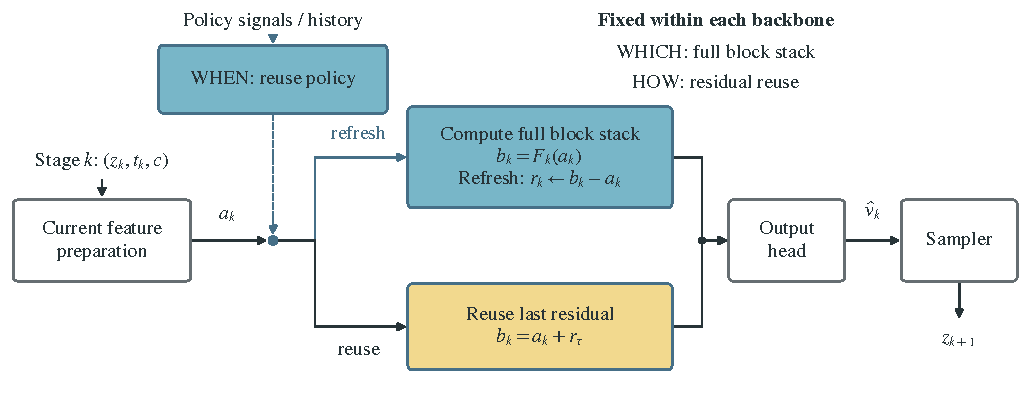
\includegraphics[width=\linewidth]{figures/caching_framework.pdf}
\caption{\textbf{The reuse decision in generation.} Each policy chooses between recomputing the transformer block stack and reusing its cached residual. Cache scope and reconstruction are shared within each backbone.}
\label{fig:framework}
\end{figure}

\FloatBarrier
\section{Benchmark}
\label{sec:benchmark}
\label{sec:methods}
\subsection{Tasks and Implementations}
We benchmark five methods in parallel text-to-video and text-to-image settings.
Table~\ref{tab:protocol} summarizes the backbones, data, sampling settings, and hardware; all methods within a task use the same settings and paired Uncached references.

\begin{table}[!htbp]
\caption{Benchmark settings for video and image generation. CFG denotes classifier-free guidance.}
\label{tab:protocol}
\centering\small
\begin{tabularx}{\linewidth}{lXX}
\toprule & Video: Wan2.1-T2V-1.3B~\cite{wan2025wan} & Image: FLUX.1-dev~\cite{flux2024}\\
\midrule
Data & 110-prompt VBench~\cite{huang2024vbench} subset; main seeds 0--4 & All 200 DrawBench~\cite{saharia2022imagen} prompts; seed 0\\
Hardware & NVIDIA A100-SXM4-80GB & NVIDIA H200\\
Output & $832\times480$, 81 frames, 16 fps & $1024\times1024$, batch size 1\\
Sampler & UniPC~\cite{zhao2023unipc}, 50 steps, CFG~\cite{ho2022cfg} 5, flow shift 5 & FlowMatch-Euler, 28 steps, guidance 3.5\\
Precision & BF16 transformer, FlashAttention2, no offload & BF16, T5 maximum length 512\\
Calibration & MagCache and SenCache: eight project Commons videos & SenCache port: 64 DOCCI~\cite{onoe2024docci} images\\
Timing & Development: warmup 1, timed 3; test: worker warmup, timed 1 per task & Warmup per configuration; paired per-image timing\\
\bottomrule
\end{tabularx}

\end{table}

Within each backbone, the cached methods share the forward path and residual-reuse operation.
At sampling stage $k$, the network predicts $v_k=f_\theta(z_k,t_k,c)$, and the sampler uses this prediction to update the latent $z_k$.
Let $a_k$ denote the block-stack input and $r_k=F_k(a_k)-a_k$ its residual.
With $\tau(k)$ denoting the most recent refresh, the block output is
\begin{equation}
 \widehat F_k(a_k)=
 \begin{cases}
 a_k+r_k,&\text{compute and refresh},\\
 a_k+r_{\tau(k)},&\text{reuse}.
 \end{cases}
\end{equation}
Thus, reuse skips the expensive block computation while preserving the sampling update.
Wan2.1 makes two classifier-free-guidance calls per sampling stage, giving 100 possible full-block calls per video; FLUX.1-dev makes one call per stage, giving 28 per image.
We report these computation counts separately from the nominal number of sampling steps.

The FLUX.1-dev versions of TeaCache, MagCache, and SeaCache derive from their authors' implementations; SenCache on FLUX.1-dev is a project adaptation of the Wan2.1 rule.
The Wan2.1 implementations use matching MagCache and SenCache profiles calibrated on eight project Commons videos.
For FLUX.1-dev, MagCache uses upstream 28-step ratios and SenCache uses a sensitivity profile calibrated on 64 DOCCI~\cite{onoe2024docci} images.
The fixed-schedule image control computes the first six stages, distributes the remaining selected computations, and includes the final stage.
This control provides a predetermined schedule for comparison.
Appendices~\ref{app:reproducibility} and~\ref{app:rules} describe retained evidence and signal details; Table~\ref{tab:guards} lists the protection rules used in the analysis.

\subsection{Evaluation Protocol}
The Wan2.1 suite contains 1,411 development tasks, 336 component-ablation tasks, and 3,750 test tasks.
The main fidelity comparison uses 550 output-reference pairs per cached method, covering 110 prompts and five seeds.
Each method also has 200 temporal-flickering candidates; these extra seeds are excluded from the main fidelity table.
The development curve uses the 86 pairs common to all 14 cached configurations, covering 29 prompts.
Video thresholds were selected on the development set to reach at least $2\times$ denoising acceleration and then frozen for testing.

The image suite contains 24 configurations and 4,800 records, using one seed for each of the 200 DrawBench prompts.
For every comparison, cached outputs and timings are paired with the corresponding Uncached run on the same prompt, seed, backbone, and hardware.
The two image timing batches produced bit-identical Uncached images, but their measured times differ, so each batch retains its own timing reference.
We compare measured operating points, meaning the observed time and quality at a particular configuration; equal numerical thresholds are not treated as equal budgets.

\subsection{Evaluation Criteria}
We distinguish reference fidelity from generated-content quality.
Peak signal-to-noise ratio (PSNR), structural similarity (SSIM)~\cite{wang2004ssim}, and learned perceptual image patch similarity (LPIPS)~\cite{zhang2018lpips} quantify deviation from the paired Uncached output.
Greater reference fidelity corresponds to increasing PSNR or SSIM, or decreasing LPIPS.
VBench~\cite{huang2024vbench} evaluates separate video properties, while CLIP similarity~\cite{radford2021clip} and ImageReward~\cite{xu2023imagereward} provide complementary automatic image assessments.
CLIPScore~\cite{hessel2021clipscore} addresses text-image compatibility, and GenEval~\cite{ghosh2023geneval} tests compositional correctness; these evaluation targets differ from reference similarity.
We use neither of those two additional evaluators in the reported experiments; our examples inspect specific content errors directly.
Uncached supplies a full-computation reference, not a guarantee that the prompt is satisfied.

Generation time includes text encoding, denoising, and variational autoencoder (VAE) decoding, and excludes model loading, policy initialization, CPU transfer, and file encoding.
Wan2.1 speedup is the ratio of total paired generation times; FLUX.1-dev speedup is the median of paired per-image ratios.
A simple cost decomposition is
\begin{equation}
T_\pi=A+\sum_j\big[c_jC_j+(1-c_j)R_j+G_j\big],
\label{eq:cost}
\end{equation}
where $c_j$ is the decision to compute at call $j$, $C_j$ and $R_j$ are compute and reuse costs, $G_j$ is decision overhead, and $A$ contains the remaining pipeline work.
The computation count therefore captures only part of measured latency.
For a time budget $B$, the comparison seeks low paired deviation $d$ under that budget:
\begin{equation}
\min_\pi\;\mathbb E[d(x_\pi,x_{\rm full})]
\quad\text{subject to}\quad\mathbb E[T_\pi]\le B.
\end{equation}
Threshold sweeps provide measured points on this speed--fidelity trade-off.

We report prompt-bootstrap intervals where available and distinguish intervals for individual means from intervals for paired differences.
The following sections first report the measured trade-offs and content assessments, then analyze the decisions that produce them.

\section{Experimental Results}
\label{sec:budgets}
\subsection{Text-to-Video Generation}
\label{sec:wan}
Table~\ref{tab:wan} reports the frozen video test configurations and their paired fidelity and runtime.
The configurations satisfy a development target for denoising acceleration, but reach different generation-time budgets.

\begin{table}[!htbp]
\caption{Wan test results on 550 paired samples per cached method. Compute (\%) is the fraction of full-block calls out of 100 per video; bold marks the lowest mean LPIPS.}
\label{tab:wan}
\centering\small\setlength{\tabcolsep}{3pt}
\renewcommand{\tabularxcolumn}[1]{m{#1}}%
\begin{tabularx}{\linewidth}{llRRRRRRR}
\toprule
\rowcolor{tabhead} & & \multicolumn{4}{c}{\thead{Efficiency}} & \multicolumn{3}{c}{\thead{Fidelity to Uncached}} \\
\cmidrule(lr){3-6}\cmidrule(l){7-9}
\rowcolor{tabhead}Method & $\epsilon$ & Time $\downarrow$ & Generation\newline speedup $\uparrow$ & Denoising\newline speedup $\uparrow$ & Compute $\downarrow$ & PSNR $\uparrow$ & SSIM $\uparrow$ & LPIPS $\downarrow$ \\
\midrule
\rowcolor{refrow}\mUnc & -- & 271.33 & 1.000 & 1.000 & 100.0 & -- & -- & -- \\
\midrule
\mTea & 0.12 & 171.52 & 1.582 & 2.369 & 42.0 & 21.80 & 0.794 & 0.1464 \\
\mMag & 0.12 & 171.48 & 1.582 & 2.370 & 42.0 & 25.30 & 0.871 & 0.0873\rel{$-$40.3\%} \\
\mSea & 0.2 & 182.53 & 1.486 & 2.058 & 48.0 & \best{29.22} & \best{0.929} & \bestlp{0.0482}\rel{$-$67.1\%} \\
\mSen & 0.5 & \best{164.84} & \best{1.646} & \best{2.606} & \best{38.2} & 22.10 & 0.800 & 0.1423\rel{$-$2.8\%} \\
\bottomrule
\end{tabularx}


\end{table}

\textbf{Speed and Fidelity.}
The thresholds were frozen using a development target of at least $2\times$
\emph{denoising} acceleration. They do not equalize test generation time.
Among the displayed cached configurations, SeaCache has the lowest LPIPS (0.0482)
at $1.486\times$ generation speedup; SenCache is
fastest at $1.646\times$, with LPIPS 0.1423. MagCache and TeaCache both execute 42 of 100
transformer calls and run at almost identical times (171.48 versus 171.52 s),
but MagCache's LPIPS is 0.0873 versus 0.1464: a 40.3\% reduction. MagCache therefore remains a strong baseline on Wan.

\begin{figure}[!htbp]
\centering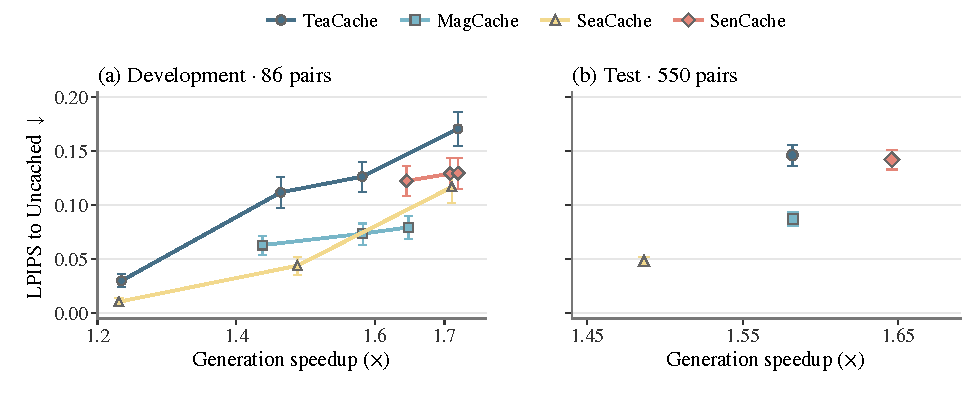
\includegraphics[width=\linewidth]{figures/wan_speed_fidelity.pdf}
\caption{\textbf{Wan speed--fidelity trade-offs.} Development and test results, with prompt-bootstrap 95\% intervals for mean LPIPS.}
\label{fig:wan}
\end{figure}
The development sweep reinforces the budget-dependent conclusion: near 165 s,
MagCache 0.24 has LPIPS 0.0795 versus SenCache 0.5's 0.1226; near 220 s, SeaCache 0.1 has
0.0105 versus TeaCache 0.04's 0.0299. These development comparisons remain separate
from the frozen test results.

\FloatBarrier
\subsection{Text-to-Image Generation}
\label{sec:flux}
Table~\ref{tab:flux} groups selected image configurations by their measured speedup, while Figure~\ref{fig:flux} shows the complete sweep.
A matched-count comparison occurs near $2.45\times$ speedup, where TeaCache, MagCache, and SenCache all compute 11 of 28 stages.

\begin{table}[!htbp]
\caption{FLUX comparisons at similar measured speedups on 200 DrawBench prompts. Suffixes give cache thresholds or Fixed computation counts; bold marks the lowest mean LPIPS within each group.}
\label{tab:flux}
\centering\small\setlength{\tabcolsep}{4pt}
\begin{tabular*}{\linewidth}{@{\extracolsep{\fill}}lrrrrrr@{}}
\toprule
Configuration & Speedup & \shortstack{PSNR $\uparrow$\\(dB)} & SSIM $\uparrow$ & LPIPS $\downarrow$ & CLIP $\uparrow$ & ImageReward $\uparrow$ \\
\midrule
\multicolumn{7}{@{}l}{\textit{Near $1.7\times$ generation speedup}} \\[2pt]
SeaCache 0.3 & 1.710 & 29.43 & 0.930 & \textbf{0.0629} & 27.62 & 1.008 \\
SenCache 0.5 & 1.719 & 28.31 & 0.920 & 0.0720 & 27.56 & 1.025 \\
Fixed 16 & 1.723 & 28.19 & 0.920 & 0.0722 & 27.59 & 1.023 \\
TeaCache 0.25 & 1.717 & 19.77 & 0.786 & 0.2317 & 27.89 & 1.049 \\
\midrule
\multicolumn{7}{@{}l}{\textit{Near $1.96\times$ generation speedup}} \\[2pt]
Fixed 14 & 1.959 & 26.37 & 0.893 & \textbf{0.1011} & 27.57 & 1.021 \\
SenCache 0.8 & 1.955 & 26.67 & 0.888 & 0.1094 & 27.55 & 1.018 \\
\midrule
\multicolumn{7}{@{}l}{\textit{Near $2.27\times$ generation speedup}} \\[2pt]
SenCache 1 & 2.262 & 25.61 & 0.875 & \textbf{0.1259} & 27.46 & 1.007 \\
Fixed 12 & 2.273 & 24.87 & 0.864 & 0.1384 & 27.53 & 1.008 \\
SeaCache 0.45 & 2.245 & 24.26 & 0.862 & 0.1401 & 27.58 & 1.007 \\
MagCache 0.09 & 2.273 & 22.42 & 0.832 & 0.1763 & 27.69 & 1.027 \\
\midrule
\multicolumn{7}{@{}l}{\textit{Near $2.45\times$ generation speedup}} \\[2pt]
SenCache 2 & 2.457 & 24.56 & 0.846 & \textbf{0.1576} & 27.49 & 1.004 \\
SeaCache 0.6 & 2.442 & 22.25 & 0.822 & 0.1930 & 27.77 & 1.014 \\
MagCache 0.12 & 2.471 & 21.82 & 0.817 & 0.1996 & 27.67 & 1.005 \\
TeaCache 0.5 & 2.450 & 17.97 & 0.727 & 0.3231 & 27.78 & 1.017 \\
\bottomrule
\end{tabular*}


\end{table}

\begin{figure}[!htbp]
\centering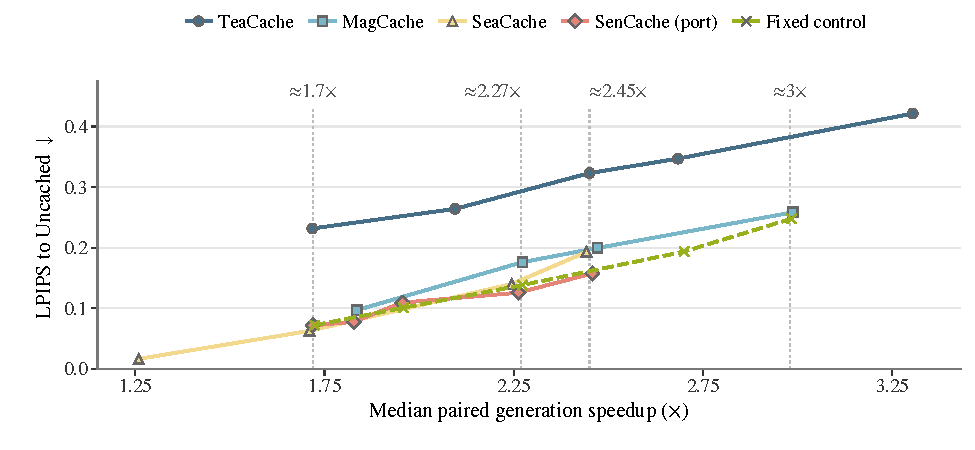
\includegraphics[width=\linewidth]{figures/flux_speed_fidelity.pdf}
\caption{\textbf{FLUX speed--fidelity trade-offs.} All measured configurations on 200 DrawBench prompts, including the fixed-schedule control.}
\label{fig:flux}
\end{figure}

\textbf{Matched-Count Comparisons.}
Near $2.45\times$, TeaCache 0.5, MagCache 0.12 and SenCache 2 each compute 11 of 28 stages
on every prompt. SenCache's mean LPIPS is 51.2\% lower than TeaCache's and 21.0\% lower
than MagCache's; their median generation times span less than 0.9\%. The paired
SenCache-minus-TeaCache LPIPS difference is $-0.16553$, with a 95\% interval
$[-0.17876,-0.15241]$; SenCache has lower LPIPS on 195 of 200 prompts.

\textbf{Budget-Dependent Comparison.}
Near $1.7\times$, SeaCache 0.3 has lower LPIPS than SenCache 0.5: the paired mean difference
is $-0.00915$, with reported 95\% interval $[-0.01271,-0.00617]$, a 12.7\%
reduction relative to SenCache.
Near $2.45\times$, SenCache 2 has lower LPIPS than SeaCache 0.6: difference $-0.03542$,
interval $[-0.04290,-0.02811]$, an 18.4\% reduction relative to SeaCache.
SenCache has lower LPIPS on 80.5\% of prompts at the faster budget.

\textbf{Adaptive and Fixed Schedules.}
The paired LPIPS interval between SenCache 0.5 and Fixed 16 includes zero
$[-0.00134,0.00107]$.
Near $1.96\times$, Fixed 14 has lower LPIPS than SenCache 0.8, while SenCache has
higher PSNR. Near $2.27\times$, SenCache 1 improves LPIPS over Fixed 12 by
0.01252 and has lower LPIPS on 93.5\% of prompts.

\subsection{Fidelity and Content Quality}
\label{sec:quality}

Table~\ref{tab:vbench} keeps the 16 VBench dimensions separate. Each uses ten
declared prompts and 50 evaluated videos per method, except color: valid counts
are 36/35/37/37/36 for Uncached/TeaCache/MagCache/SeaCache and SenCache. Color averages therefore have
different detection-valid subsets. Prompts overlap across dimensions.

\begin{table}[!htbp]
\caption{VBench scores across 16 dimensions on the evaluated subset. Color uses method-dependent valid sets; dynamic degree measures motion prevalence.}
\label{tab:vbench}
\centering\small\setlength{\tabcolsep}{4pt}
\renewcommand{\tabularxcolumn}[1]{m{#1}}%
\begin{tabularx}{\linewidth}{lRRRRR}
\toprule
\rowcolor{tabhead}Dimension & \mUnc & \mTea & \mMag & \mSea & \mSen \\
\midrule
\grouprow{6}{Video quality}
Subject consistency & \cellcolor{refrow}0.9611 & 0.9630 & 0.9623 & 0.9617 & 0.9622 \\
Background consistency & \cellcolor{refrow}0.9804 & 0.9805 & 0.9794 & 0.9797 & 0.9804 \\
Temporal flickering & \cellcolor{refrow}0.9894 & 0.9880 & 0.9874 & 0.9875 & 0.9877 \\
Motion smoothness & \cellcolor{refrow}0.9805 & 0.9809 & 0.9809 & 0.9808 & 0.9808 \\
Dynamic degree & \cellcolor{refrow}0.7200 & 0.6800 & 0.7000 & 0.7000 & 0.6800 \\
Aesthetic quality & \cellcolor{refrow}0.6566 & 0.6534 & 0.6500 & 0.6515 & 0.6502 \\
Imaging quality & \cellcolor{refrow}0.6720 & 0.6627 & \loss{0.6598} & 0.6656 & 0.6628 \\
\midrule
\grouprow{6}{Video--condition consistency}
Object class & \cellcolor{refrow}0.7462 & \gain{0.7588} & \gain{0.7775} & \gain{0.7712} & \gain{0.7812} \\
Multiple objects & \cellcolor{refrow}0.6887 & \loss{0.6687} & 0.6800 & 0.6825 & \gain{0.7013} \\
Human action & \cellcolor{refrow}0.7600 & \gain{0.7800} & 0.7600 & 0.7600 & \gain{0.8000} \\
Color & \cellcolor{refrow}0.9373 & \gain{0.9538} & 0.9344 & 0.9429 & \gain{0.9516} \\
Spatial relationship & \cellcolor{refrow}0.8111 & \loss{0.7556} & \loss{0.7615} & \loss{0.7599} & \loss{0.7507} \\
Scene & \cellcolor{refrow}0.0862 & \loss{0.0600} & 0.0850 & \loss{0.0638} & \loss{0.0587} \\
Appearance style & \cellcolor{refrow}0.2042 & 0.2020 & 0.2022 & 0.2024 & 0.2024 \\
Temporal style & \cellcolor{refrow}0.2369 & 0.2387 & 0.2373 & 0.2368 & 0.2383 \\
Overall consistency & \cellcolor{refrow}0.2088 & 0.2087 & 0.2066 & 0.2071 & 0.2083 \\
\bottomrule
\end{tabularx}


\end{table}

SeaCache's stronger reference fidelity does not make it best on every VBench dimension.
For example, spatial-relationship scores fall from Uncached's 0.8111 to
0.7507--0.7615 for the cached methods, whereas object-class scores are higher.
Subject consistency and motion smoothness differ only slightly.
In FLUX near $2.45\times$, SenCache's lower LPIPS coexists with lower CLIP than SeaCache
(27.49 versus 27.77), further illustrating distinct evaluation targets.

\begin{figure}[!htbp]
\centering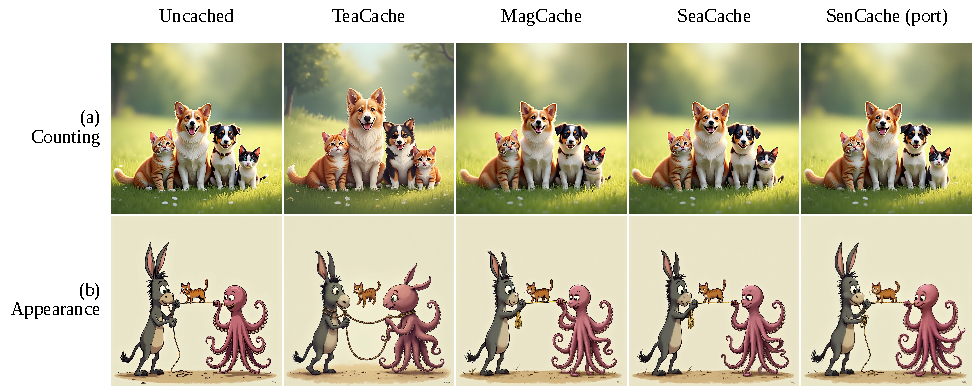
\includegraphics[width=\linewidth]{figures/flux_cases_restyled.pdf}
\caption{\textbf{Reference fidelity and prompt correctness.} DrawBench examples near $2.45\times$ speedup. Top: Uncached depicts two cats and two dogs despite the requested three of each. Bottom: TeaCache alters the octopus-like character's appearance and pose.}
\label{fig:fluxcases}
\end{figure}

\FloatBarrier
\begin{figure}[!htbp]
\centering
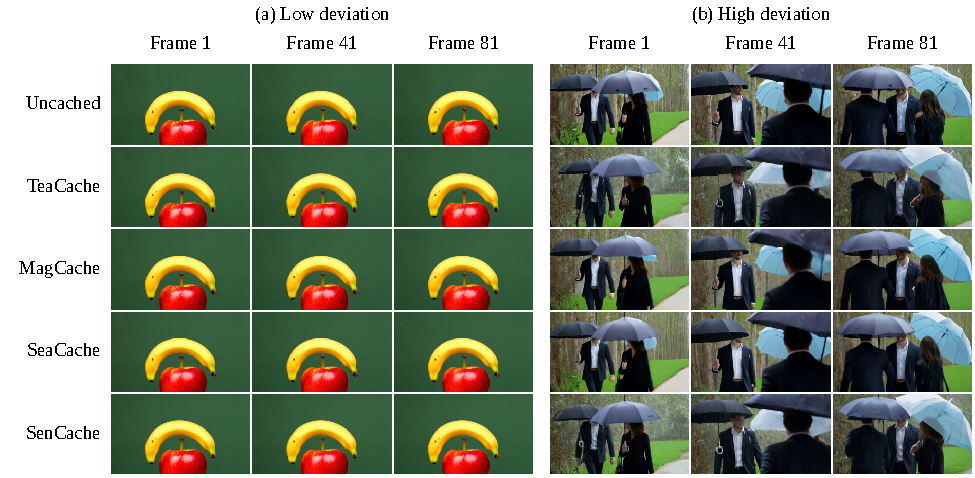
\includegraphics[width=\linewidth]{figures/wan_cases_restyled.pdf}
\caption{\textbf{Low- and high-deviation video cases.} Frames 1, 41, and 81 from LPIPS-selected cases, with seed 2 and settings from Table~\ref{tab:wan}. Left: the fruit arrangement is largely preserved. Right: people and umbrellas change; SeaCache remains closest to Uncached.}
\label{fig:wancases}
\end{figure}

The image panels are selected from four retained examples.
The video panels show the pairs with the lowest worst-method LPIPS and highest mean LPIPS, respectively, among 550 pairs.
The examples show both preservation of reference errors and changes introduced by caching.
Reference fidelity is therefore a useful measure of acceleration-induced change, but it cannot establish prompt correctness by itself.
The next section examines how the decision signals and protection rules produce the measured computation patterns.

\FloatBarrier
\section{Analysis of Caching Decisions}
\label{sec:mechanism}
\subsection{Component Ablations}
\label{sec:ablation}

SeaCache and SenCache ablations use 21 and 24 paired samples from seven and eight prompts, respectively.
We compare the resulting speed--fidelity curves because removing a component can change both reuse frequency and output deviation.

\begin{figure}[!htbp]
\centering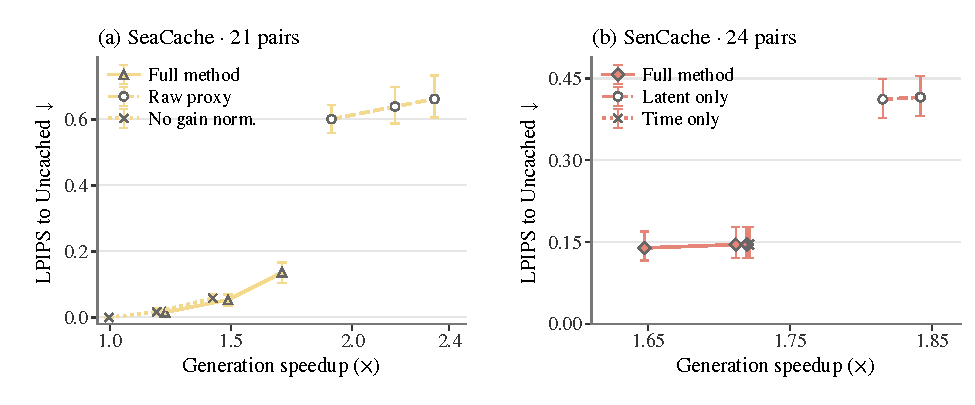
\includegraphics[width=\linewidth]{figures/wan_component_tradeoffs.pdf}
\caption{\textbf{Component ablations on Wan.} Speed--fidelity curves with prompt-bootstrap 95\% intervals for mean LPIPS.}
\label{fig:ablation}
\end{figure}

\begin{table}[!htbp]
\caption{Selected Wan component-ablation results. Full and ablated variants share the same evaluation pairs within each method.}
\label{tab:ablation}
\centering\small\setlength{\tabcolsep}{4pt}
\renewcommand{\tabularxcolumn}[1]{m{#1}}%
\begin{tabularx}{\linewidth}{lrRRR}
\toprule
\rowcolor{tabhead}Variant & $\epsilon$ & Speedup $\uparrow$ & LPIPS $\downarrow$ & Compute $\downarrow$ \\
\midrule
\grouprow{5}{\mSea}
\rowcolor{refrow}Full & 0.1 & 1.229 & 0.0153 & 70.1 \\
No gain norm. & 0.1 & \loss{0.998} & \gain{0.0000} & 100.0 \\
Raw proxy & 0.1 & \gain{1.914} & \loss{0.6008} & 24.6 \\
\addlinespace[2pt]
\rowcolor{refrow}Full & 0.2 & 1.488 & 0.0532 & 47.8 \\
No gain norm. & 0.2 & \loss{1.194} & \gain{0.0169} & 74.0 \\
Raw proxy & 0.2 & \gain{2.176} & \loss{0.6389} & 14.7 \\
\midrule
\grouprow{5}{\mSen}
\rowcolor{refrow}Full & 0.5 & 1.647 & 0.1394 & 38.0 \\
Latent only & 0.5 & \gain{1.815} & \loss{0.4120} & 29.2 \\
Time only & 0.5 & 1.721 & 0.1457 & 34.0 \\
\addlinespace[2pt]
\rowcolor{refrow}Full & 2 & 1.719 & 0.1457 & 34.0 \\
Latent only & 2 & \gain{1.842} & \loss{0.4158} & 28.0 \\
Time only & 2 & 1.721 & 0.1457 & 34.0 \\
\bottomrule
\end{tabularx}


\end{table}

\textbf{SeaCache: Gain Normalization.}
This ablation tests whether the spectral comparison remains on a useful decision scale when normalization is removed.
At threshold 0.1, removing gain normalization eliminates reuse: compute rate 100\%, LPIPS 0, and approximately baseline runtime.
The zero deviation therefore indicates full computation, not an improved caching trade-off.
At 0.2, the ablated variant still computes 74.0\% of transformer calls, compared with 47.8\% for the full method.
Using the raw proxy instead produces $1.91$--$2.34\times$ speedup but LPIPS 0.601--0.662 over the tested thresholds.
The transformation changes the gate's effective operating range in both directions: removing normalization suppresses reuse, whereas the raw proxy permits substantially more deviation at the tested settings.
These variants show how normalization and the comparison proxy shape the decision scale and the resulting speed--fidelity trade-off.

\textbf{SenCache: Latent and Time Signals.}
The signal-removal ablation tests the contribution of the two terms used to estimate change since the last refresh.
At threshold 0.5, the latent-only variant is faster but has LPIPS 0.4120, compared with 0.1394 for the full rule.
At thresholds 2 and 4, the full and time-only variants converge to approximately 0.1457 LPIPS and 34\% compute rate.
We next inspect FLUX decision traces to determine when protection rules control refreshes.

\FloatBarrier
\subsection{Computation Placement}
\label{sec:math}
The ablations show that changing a signal can change the compute rate. To explain
the reuse decisions, we must also inspect where those computations occur. Figure~\ref{fig:schedules}
shows the dominant sequences, including their prevalence across prompts.
\begin{figure}[!htbp]
\centering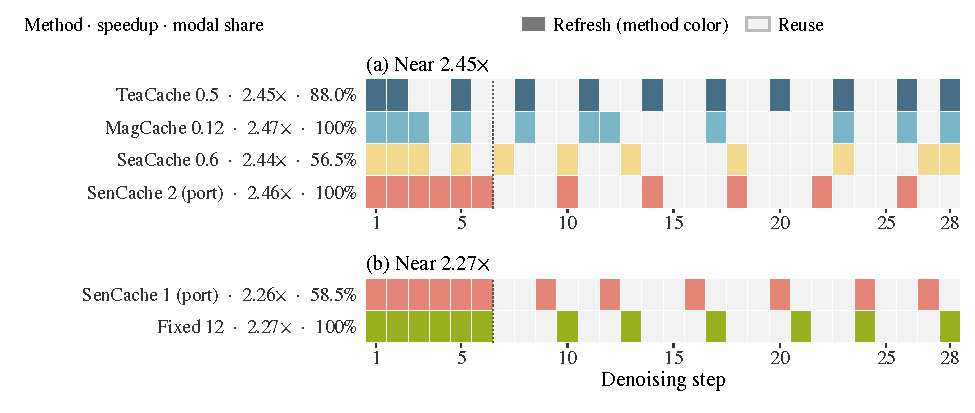
\includegraphics[width=\linewidth]{figures/flux_modal_schedules.pdf}
\caption{\textbf{Computation placement in FLUX.} Colored cells denote compute and pale cells reuse. Each row gives the most frequent schedule and its coverage among 200 prompts; the dotted line marks stage six.}
\label{fig:schedules}
\end{figure}

\textbf{Proposition 1: Equal computation counts do not determine final error.}
Consider $x_{k+1}=x_k+v_k/4$, $x_0=0$, with residual reuse equal to velocity reuse
(zero stem and identity head). Using $C$ for computation and $R$ for reuse, schedules $A=(C,C,R,C)$ and $B=(C,R,C,C)$ both
compute three times, protect both endpoints and have no consecutive reuses.
For velocities $(0,1,1,1)$, full computation and $A$ end at $3/4$, but $B$ ends
at $1/2$. For $(0,0,1,1)$, full computation and $B$ end at $1/2$, but $A$ ends
at $1/4$. Direct summation proves both unequal errors and reversal of the
preferred schedule. With equal operation costs, runtime is also equal.
This construction demonstrates that computation placement can change the final error even at the same computation cost.

The FLUX traces show different computation schedules near $2.45\times$, where TeaCache, MagCache and SenCache each compute eleven stages but attain different LPIPS values (Table~\ref{tab:flux}).

\subsection{Reuse Constraints}
\label{sec:guards}
The fixed-control results already show that online input dependence is not
sufficient for better LPIPS. A stronger question is whether the gate is still
choosing refreshes, or a guard has taken over. The following two propositions
make this distinction precise for a fixed implementation and audited inputs.
Table~\ref{tab:guards} specifies the implemented protection rules that constrain those decisions.

\begin{table}[!htbp]
\caption{Protection rules used by each policy. $K$ denotes the maximum number of consecutive reuses.}
\label{tab:guards}
\centering\small\setlength{\tabcolsep}{5pt}
\begin{tabularx}{\linewidth}{@{}lXX@{}}
\toprule
Policy & Wan: 50 sampling stages & FLUX: 28 sampling stages\\
\midrule
TeaCache / SeaCache & First and last stages compute; no explicit reuse cap.
& First and last stages compute; no explicit reuse cap.\\[3pt]
MagCache & First ten stages compute; $K=4$.
& First three stages and stage 12 compute; $K=5$.\\[3pt]
SenCache & First ten stages use $\epsilon_{\rm early}=0.045$; $K=3$.
& First six stages use $\epsilon_{\rm early}=0.045$; $K=3$.\\[3pt]
Fixed & Not tested in this study.
& First six stages forced; remaining computes distributed, including the last.\\
\bottomrule
\end{tabularx}
\end{table}

\textbf{Proposition 2: A maximum-reuse cap gives a tight count bound.}
For $N$ sampling stages containing $M$ full computations, if the first stage computes and at most $K$ consecutive reuses are allowed,
$N\le M(K+1)$, so $M\ge\lceil N/(K+1)\rceil$ computes are necessary. Conditional
on the first $g$ stages all computing, the tighter bound is
\begin{equation}
M\ge g+\left\lfloor\frac{N-g}{K+1}\right\rfloor.\label{eq:count}
\end{equation}
For $c$ additional computes, at most $c+1$ reuse runs remain, hence
$N-g\le c+(c+1)K$. Writing $N-g=q(K+1)+r$, $0\le r\le K$, the sequence
$C^g(R^KC)^qR^r$ attains the bound. For all 200 FLUX.1-dev records with SenCache at threshold 2,
$N=28$, $K=3$, and the \emph{observed} $g=6$ prefix gives the attained minimum
$M=11$. The early threshold is 0.045; six computes are not hard-coded.
Without that observed prefix the bound is seven, not eleven.

\textbf{Proposition 3: Logged decisions can certify a threshold interval.}
Fix inputs, initial noise, weights, implementation, profiles, early threshold
and $K$. Assume deterministic execution and that the varied main threshold
only affects the post-prefix gate. Across all audited post-prefix events, let $L$ be the largest normalized error at
a reuse and $U$ the smallest at an unforced refresh, with $L=-\infty$ or $U=\infty$
when the corresponding event set is empty.
Every $\epsilon\in(L,U]$ preserves the path: by induction, identical previous
decisions give identical states and errors; the strict comparison
$e_k<\epsilon$ keeps each reuse/refresh decision, and cap-forced refreshes remain
forced. The early prefix is unchanged.

The traces contain 3,400 post-prefix reuses and 1,000 cap-forced refreshes.
The largest reuse score is $L=1.606399434983263$, with no unforced refresh, so $U=\infty$.
Therefore, any main threshold $\epsilon\ge1.607$ preserves these logged schedules under the stated assumptions.

\FloatBarrier
\subsection{Generation Efficiency}
Equation~\ref{eq:cost} explains why nominal skips are only a cost proxy.
Wan's Uncached mean is 271.33 s: 172.74 s of denoising and a 98.59 s remainder.
Applying Amdahl's law~\cite{amdahl1967validity}, if that remainder $A$ is fixed and denoising $D$ is accelerated by $r$, then
\begin{equation}
 S(r)=\frac{A+D}{A+D/r},\qquad
 \lim_{r\rightarrow\infty}S(r)=\frac{A+D}{A}\simeq2.75.
\end{equation}
SeaCache's $2.06\times$ denoising gain thus becomes $1.49\times$ generation speedup.
This decomposition connects the computation-level analysis to the generation time measured by the benchmark.

\clearpage
\section{Discussion}
\label{sec:discussion}
\subsection{Comparative Findings}
The equal-count, near-equal-latency comparisons establish that the choice of policy has a substantial effect on reference fidelity even when the amount of full-block computation is held constant.
This effect is observed in both tasks, although the strongest measured policy differs between the settings and budgets.
Table~\ref{tab:strengths} summarizes these observed strengths and limitations.
The comparisons evaluate complete policies, including their signals and protection rules; they do not identify a single component or refresh position as the cause of each gap.

\begin{table}[!htbp]
\caption{Strengths and limitations observed in the benchmark comparisons.}
\label{tab:strengths}
\centering\small\setlength{\tabcolsep}{5pt}
\begin{tabularx}{\linewidth}{@{}lXX@{}}
\toprule
Method & Observed strength & Observed limitation\\
\midrule
TeaCache & Reduces generation time in both tasks. & Larger LPIPS than MagCache on the equal-count Wan comparison and than SenCache at the matched-count FLUX point.\\[3pt]
MagCache & Lower Wan LPIPS than TeaCache at the same compute count and almost identical time. & Higher LPIPS than SenCache at the matched-count FLUX point; magnitude profiles must match the generation configuration.\\[3pt]
SeaCache & Lowest LPIPS at the shown Wan test settings; lower LPIPS than SenCache near $1.7\times$ on FLUX. & The Wan advantage comes with more generation time; SenCache has lower LPIPS near $2.45\times$ on FLUX.\\[3pt]
SenCache & Lowest LPIPS among the compared FLUX policies near $2.45\times$. & The FLUX result is a project port; its fast schedule is guard-limited on the audited inputs, and the Wan sweep does not dominate MagCache.\\
\bottomrule
\end{tabularx}
\end{table}

Uncached defines the fidelity target, not a guarantee of correct content.
The counting example preserves an error already present in the reference, while the FLUX LPIPS and CLIP comparisons prefer different policies at the fast budget.
Reference fidelity therefore answers whether acceleration changes the generator's output; content assessment answers whether that output satisfies the prompt.
A claim of better generation quality requires the latter evidence as well.

\subsection{Tuning and Extensions}
Threshold tuning should target measured generation time and reference fidelity, with the realized schedule inspected alongside both.
The component ablations show why the threshold value alone is insufficient: changing normalization or removing a signal changes the scale of the gate and the resulting compute rate.
The SenCache trace audit identifies a different limit: once the consecutive-reuse cap determines every post-prefix refresh, relaxing the main threshold cannot reduce the compute count on those audited inputs.

These observations motivate two untested extensions.
First, replaying a certified schedule could remove repeated gate evaluation while preserving the same decisions for the certified inputs.
Second, the propagation model in Appendix~\ref{app:propagation} motivates allocating different local error budgets across stages, rather than applying a uniform tolerance to errors with different downstream effects.
This connects the propagation analysis to dynamic-threshold ideas considered in SenCache~\cite{haghighi2026sencache}.

\subsection{Limitations}
Wan test timing has one repeat per task, compared with three in development; FLUX uses one seed per prompt, and the VBench subset is small.
Prompt-bootstrap comparisons are exploratory, without multiple-comparison correction.
The early-prefix and threshold-plateau conclusions are conditional on the audited inputs and implementation, with some historical profile and guard provenance reconstructed retrospectively.
Full raw images and frames were not retained, so the saved metrics and selected cases support analysis but not complete metric recomputation.
The study does not evaluate maximum-reuse-cap, early-threshold, or calibration-size sweeps, or equal-time reduced-step controls.

\FloatBarrier
\section{Conclusion}
Our five-method benchmark evaluates temporal caching policies in image and video generation.
At equal computation counts and nearly identical latency, MagCache lowers Wan LPIPS by 40.3\% relative to TeaCache, while SenCache lowers FLUX LPIPS by 51.2\%.
The lower-LPIPS choice between SeaCache and SenCache reverses across two measured FLUX budgets.
At the analyzed SenCache setting, all 200 prompts use the same 11-computation schedule over 28 steps.
The consecutive-reuse limit forces every refresh after the early stages, preventing larger main thresholds from reducing computation further.
These results establish the need to examine both the placement of computation and the constraints on reuse, beyond skip counts.


\clearpage
\setlength{\bibsep}{1pt}
{\small
\bibliographystyle{plainnat}
\bibliography{references}
}
\appendix
\section*{Appendix}
\section{A conditional propagation model}
\label{app:propagation}
This appendix relates local caching error to accumulated latent error.
Let full and cached Euler trajectories start from the same state:
\begin{align}
 z_{k+1}&=z_k+h_k v_k(z_k),\\
 \widetilde z_{k+1}&=\widetilde z_k+h_k\{v_k(\widetilde z_k)+\delta_k\}.
\end{align}
Here $\delta_k=\widetilde v_k(\widetilde z_k)-v_k(\widetilde z_k)$ is the local
cache error \emph{at the cached state}, separated from accumulated trajectory
error. If $v_k$ is $L_k$-Lipschitz on the relevant region and
$\|\delta_k\|\le d_k$, the triangle inequality gives
\begin{equation}
E_{k+1}\le(1+|h_k|L_k)E_k+|h_k|d_k,\qquad
E_k=\|\widetilde z_k-z_k\|.
\end{equation}
Since $E_0=0$, induction yields
\begin{equation}
E_N\le\sum_{k=0}^{N-1}|h_k|d_k
              \prod_{j=k+1}^{N-1}(1+|h_j|L_j).
\label{eq:prop}
\end{equation}
Let $e_k$ be the cached residual minus the fresh residual evaluated at the same current cached state.
If the output head is $L_{H,k}$-Lipschitz, then $\|\delta_k\|\le L_{H,k}\|e_k\|$, so one may take $d_k=L_{H,k}\|e_k\|$.
For Wan's two-branch CFG with scale $s$, one may instead take
$d_k=|1-s|L_{H,u,k}\|e_{u,k}\|+|s|L_{H,c,k}\|e_{c,k}\|$.
FLUX embedded guidance does not use that two-forward CFG construction.

Equation~\ref{eq:prop} weights each local error by its step size and downstream sensitivity, making its contribution to the bound position-dependent.
For Wan's multistep UniPC sampler, augment the state with the required history and assume
the one-step augmented map obeys
$\|\widetilde Y_{k+1}-Y_{k+1}\|\le A_k\|\widetilde Y_k-Y_k\|+B_kd_k$.
The analogous bound is $\sum_k B_kd_k\prod_{j>k}A_j$. These symbolic bounds concern latent error; numerical constants and their relation to perceptual metrics are not estimated here.

\section{Reproducibility and retained evidence}
\label{app:reproducibility}

The repository records the code, model and dependency versions used in each experiment.
The submission includes the implementations, experiment configurations, calibration profiles, result summaries, report-generation scripts and SenCache decision traces.

The measurement boundary includes text encoding, denoising and VAE decoding,
but excludes model loading, policy initialization, CPU transfer and disk encoding.
Wan makes two transformer calls per sampling stage, with separate conditional
and unconditional residual caches. TeaCache, SeaCache and MagCache maintain branch-specific
decision states; SenCache applies its conditional decision to both branches. Compute
fractions count full-block calls over all calls. FLUX makes one call per stage.

The scripts in \texttt{report/README.md} rebuild tables, figures and the audit
from retained records without GPU generation. Full metric recomputation requires
the unretained pixels.

\section{Implemented signals and protection rules}
\label{app:rules}
Table~\ref{tab:guards} in Section~\ref{sec:guards} records the implemented protection rules using one-based stage indices.
The signal details below supplement that comparison. MagCache and SenCache use the existing matching
eight-video project profiles on Wan; FLUX MagCache uses upstream 28-step ratios and
SenCache uses a 64-image DOCCI sensitivity profile. TeaCache retains upstream fitted
polynomials, and SeaCache uses a scheduler-dependent spectral prior without project
data calibration. SeaCache's frequency gain is mean-normalized; its filter exponent
is three on Wan and two on FLUX. A guarded boundary call stores the raw proxy,
so the first unguarded SeaCache comparison has a raw-to-filtered transition.


Following the sensitivity criterion of SenCache~\cite{haghighi2026sencache}, our implementation uses the normalized score
\begin{equation}
\widehat e_k=\frac{J_z(\tau)\|z_k-z_\tau\|_2+
J_t(\tau)|t_k-t_\tau|}{\sqrt{D}},
\end{equation}
where $D$ is the number of latent elements and $\tau$ is the last refresh.
Sensitivity weights are selected at refresh from the nearest calibrated time
and held until the next refresh. The gate reuses when $\widehat e_k<\epsilon_k$
and the preceding reuse count is below $K$. These finite-difference sensitivity
estimates are not certified global derivative bounds.

\end{document}
